\textbf{Phần 1. Trắc nghiệm lựa chọn (Học sinh quan sát hình và chọn đáp án đúng)}
\setcounterpageref{ex}{0}

% --- CÂU 1 ---
\begin{ex} %[1D1N04]
Đếm số quả táo ở hai bên và chọn dấu thích hợp điền vào ô tròn:
\begin{center}
\begin{tikzpicture}[scale=0.75, baseline=(current bounding box.center)]
  % 5 quả táo bên trái
  \draw[fill=red!10, draw=red!60, line width=1pt] (-3,0) ellipse (2cm and 0.5cm);
  \foreach \x in {-4.2, -3.6, -3.0, -2.4, -1.8} {
    \fill[red!85!black] (\x, 0.1) circle (0.24cm);
    \fill[green!70!black] (\x, 0.34) circle (0.06cm);
  }
  \node[font=\bfseries] at (-3, -0.8) {5 quả};

  % Ô tròn so sánh
  \draw[fill=yellow!25, draw=orange!80!black, line width=1.3pt] (0, 0.1) circle (0.45cm);
  \node[font=\Large\bfseries, text=red] at (0, 0.1) {?};

  % 3 quả táo bên phải
  \draw[fill=red!10, draw=red!60, line width=1pt] (3,0) ellipse (1.6cm and 0.5cm);
  \foreach \x in {2.2, 3.0, 3.8} {
    \fill[red!85!black] (\x, 0.1) circle (0.24cm);
    \fill[green!70!black] (\x, 0.34) circle (0.06cm);
  }
  \node[font=\bfseries] at (3, -0.8) {3 quả};
\end{tikzpicture}
\end{center}
\choice
{$<$}
{\True $>$}
{$=$}
{Không có dấu}
\loigiai{
Vì $5$ quả táo nhiều hơn $3$ quả táo nên $5 > 3$.\\
Dấu thích hợp là dấu $>$.\\
\textbf{Đáp án của câu hỏi là B}
}
\end{ex}

% --- CÂU 2 ---
\begin{ex} %[1D1N04]
Đếm số bông hoa ở hai bên và chọn dấu thích hợp điền vào ô tròn:
\begin{center}
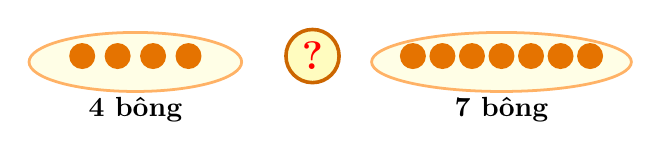
\begin{tikzpicture}[scale=0.75, baseline=(current bounding box.center)]
  % 4 bông hoa
  \draw[fill=yellow!10, draw=orange!60, line width=1pt] (-3,0) ellipse (1.8cm and 0.5cm);
  \foreach \x in {-3.9, -3.3, -2.7, -2.1} { \fill[orange!90!black] (\x, 0.1) circle (0.22cm); }
  \node[font=\bfseries] at (-3, -0.8) {4 bông};

  \draw[fill=yellow!25, draw=orange!80!black, line width=1.3pt] (0, 0.1) circle (0.45cm);
  \node[font=\Large\bfseries, text=red] at (0, 0.1) {?};

  % 7 bông hoa
  \draw[fill=yellow!10, draw=orange!60, line width=1pt] (3.2,0) ellipse (2.2cm and 0.5cm);
  \foreach \x in {1.7, 2.2, 2.7, 3.2, 3.7, 4.2, 4.7} { \fill[orange!90!black] (\x, 0.1) circle (0.22cm); }
  \node[font=\bfseries] at (3.2, -0.8) {7 bông};
\end{tikzpicture}
\end{center}
\choice
{$>$}
{\True $<$}
{$=$}
{Không có dấu}
\loigiai{
Vì $4$ bông hoa ít hơn $7$ bông hoa nên $4 < 7$.\\
Dấu thích hợp là dấu $<$.\\
\textbf{Đáp án của câu hỏi là B}
}
\end{ex}

% --- CÂU 3 ---
\begin{ex} %[1D1H04]
Chọn dấu thích hợp điền vào chỗ chấm: $8 \dots 8$.
\begin{center}
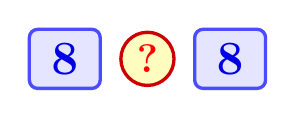
\begin{tikzpicture}[scale=0.75, baseline=(current bounding box.center)]
  \draw[fill=blue!10, draw=blue!70, line width=1.2pt, rounded corners=3pt] (-2,-0.4) rectangle (-0.8,0.6);
  \node[font=\LARGE\bfseries, text=blue!90!black] at (-1.4, 0.1) {8};

  \draw[fill=yellow!25, draw=red!80!black, line width=1.2pt] (0, 0.1) circle (0.45cm);
  \node[font=\Large\bfseries, text=red] at (0, 0.1) {?};

  \draw[fill=blue!10, draw=blue!70, line width=1.2pt, rounded corners=3pt] (0.8,-0.4) rectangle (2,0.6);
  \node[font=\LARGE\bfseries, text=blue!90!black] at (1.4, 0.1) {8};
\end{tikzpicture}
\end{center}
\choice
{\True $=$}
{$>$}
{$<$}
{Không có dấu}
\loigiai{
Hai số giống nhau nên $8 = 8$.\\
\textbf{Đáp án của câu hỏi là A}
}
\end{ex}

% --- CÂU 4 ---
\begin{ex} %[1D1H04]
Trong các chú vịt mang số $3, 8, 5, 2$, chú vịt nào mang số \textbf{lớn nhất}?
\begin{center}
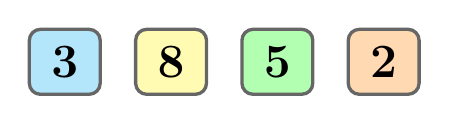
\begin{tikzpicture}[scale=0.75, baseline=(current bounding box.center)]
  \foreach \i/\num/\c in {0/3/cyan, 1/8/yellow, 2/5/green, 3/2/orange} {
    \draw[fill=\c!30, draw=black!60, line width=1.2pt, rounded corners=4pt] (\i*1.8,-0.4) rectangle (\i*1.8+1.2,0.7);
    \node[font=\LARGE\bfseries] at (\i*1.8+0.6, 0.15) {\num};
  }
\end{tikzpicture}
\end{center}
\choice
{$5$}
{$3$}
{$2$}
{\True $8$}
\loigiai{
So sánh các số: $8 > 5 > 3 > 2$. Số lớn nhất là số $8$.\\
\textbf{Đáp án của câu hỏi là D}
}
\end{ex}

% --- CÂU 5 ---
\begin{ex} %[1D1H04]
Trong các quả bóng bay mang số $6, 1, 9, 4$, quả bóng nào mang số \textbf{bé nhất}?
\begin{center}
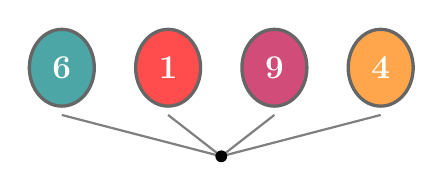
\begin{tikzpicture}[scale=0.75, baseline=(current bounding box.center)]
  \foreach \x/\num/\c in {-2.7/6/teal, -0.9/1/red, 0.9/9/purple, 2.7/4/orange} {
    \draw[line width=0.8pt, gray] (\x,-0.8) -- (0,-1.5);
    \draw[fill=\c!70, draw=black!60, line width=1.2pt] (\x,0) ellipse (0.55cm and 0.65cm);
    \node[font=\large\bfseries, text=white] at (\x,0) {\num};
  }
  \fill[black] (0,-1.5) circle (0.1cm);
\end{tikzpicture}
\end{center}
\choice
{$4$}
{$6$}
{\True $1$}
{$9$}
\loigiai{
So sánh các số: $1 < 4 < 6 < 9$. Số bé nhất là số $1$.\\
\textbf{Đáp án của câu hỏi là C}
}
\end{ex}

% --- CÂU 6 ---
\begin{ex} %[1D1H04]
Điền dấu thích hợp vào ô trống: $0 \dots 2$.
\begin{center}
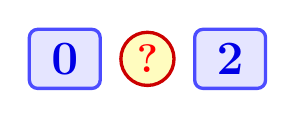
\begin{tikzpicture}[scale=0.75, baseline=(current bounding box.center)]
  \draw[fill=blue!10, draw=blue!70, line width=1.2pt, rounded corners=3pt] (-2,-0.4) rectangle (-0.8,0.6);
  \node[font=\LARGE\bfseries, text=blue!90!black] at (-1.4, 0.1) {0};

  \draw[fill=yellow!25, draw=red!80!black, line width=1.2pt] (0, 0.1) circle (0.45cm);
  \node[font=\Large\bfseries, text=red] at (0, 0.1) {?};

  \draw[fill=blue!10, draw=blue!70, line width=1.2pt, rounded corners=3pt] (0.8,-0.4) rectangle (2,0.6);
  \node[font=\LARGE\bfseries, text=blue!90!black] at (1.4, 0.1) {2};
\end{tikzpicture}
\end{center}
\choice
{$>$}
{$=$}
{\True $<$}
{Không có dấu}
\loigiai{
$0$ bé hơn mọi số tự nhiên khác $0$, do đó $0 < 2$.\\
\textbf{Đáp án của câu hỏi là C}
}
\end{ex}

% --- CÂU 7 ---
\begin{ex} %[1D1V04]
Điền dấu thích hợp vào ô trống: $10 \dots 9$.
\begin{center}
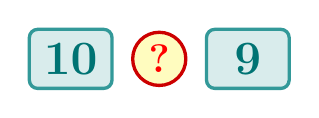
\begin{tikzpicture}[scale=0.75, baseline=(current bounding box.center)]
  \draw[fill=teal!15, draw=teal!80, line width=1.2pt, rounded corners=3pt] (-2.2,-0.4) rectangle (-0.8,0.6);
  \node[font=\LARGE\bfseries, text=teal!90!black] at (-1.5, 0.1) {10};

  \draw[fill=yellow!25, draw=red!80!black, line width=1.2pt] (0, 0.1) circle (0.45cm);
  \node[font=\Large\bfseries, text=red] at (0, 0.1) {?};

  \draw[fill=teal!15, draw=teal!80, line width=1.2pt, rounded corners=3pt] (0.8,-0.4) rectangle (2.2,0.6);
  \node[font=\LARGE\bfseries, text=teal!90!black] at (1.5, 0.1) {9};
\end{tikzpicture}
\end{center}
\choice
{$<$}
{$=$}
{Không có dấu}
{\True $>$}
\loigiai{
Vì $10 > 9$ nên điền dấu $>$.\\
\textbf{Đáp án của câu hỏi là D}
}
\end{ex}

% --- CÂU 8 ---
\begin{ex} %[1D1V04]
Sắp xếp các số $3, 7, 2, 8$ theo thứ tự từ \textbf{bé đến lớn}:
\begin{center}
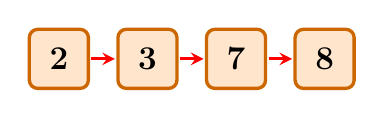
\begin{tikzpicture}[scale=0.75, baseline=(current bounding box.center)]
  \foreach \i/\num in {0/2, 1/3, 2/7, 3/8} {
    \draw[fill=orange!20, draw=orange!80!black, line width=1.2pt, rounded corners=3pt] (\i*1.5,-0.4) rectangle (\i*1.5+1.0,0.6);
    \node[font=\large\bfseries] at (\i*1.5+0.5, 0.1) {\num};
    \ifnum\i<3
      \draw[->, >=stealth, line width=1pt, red] (\i*1.5+1.05,0.1) -- (\i*1.5+1.45,0.1);
    \fi
  }
\end{tikzpicture}
\end{center}
\choice
{\True $2, 3, 7, 8$}
{$8, 7, 3, 2$}
{$2, 7, 3, 8$}
{$3, 2, 7, 8$}
\loigiai{
Từ bé đến lớn: $2 < 3 < 7 < 8$.\\
\textbf{Đáp án của câu hỏi là A}
}
\end{ex}

% --- CÂU 9 ---
\begin{ex} %[1D1V04]
Sắp xếp các số $9, 4, 6, 1$ theo thứ tự từ \textbf{lớn đến bé}:
\begin{center}
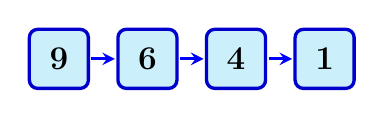
\begin{tikzpicture}[scale=0.75, baseline=(current bounding box.center)]
  \foreach \i/\num in {0/9, 1/6, 2/4, 3/1} {
    \draw[fill=cyan!20, draw=blue!80!black, line width=1.2pt, rounded corners=3pt] (\i*1.5,-0.4) rectangle (\i*1.5+1.0,0.6);
    \node[font=\large\bfseries] at (\i*1.5+0.5, 0.1) {\num};
    \ifnum\i<3
      \draw[->, >=stealth, line width=1pt, blue] (\i*1.5+1.05,0.1) -- (\i*1.5+1.45,0.1);
    \fi
  }
\end{tikzpicture}
\end{center}
\choice
{$1, 4, 6, 9$}
{$9, 4, 6, 1$}
{\True $9, 6, 4, 1$}
{$6, 9, 4, 1$}
\loigiai{
Từ lớn đến bé: $9 > 6 > 4 > 1$.\\
\textbf{Đáp án của câu hỏi là C}
}
\end{ex}

% --- CÂU 10 ---
\begin{ex} %[1D1V04]
Số thích hợp điền vào ô trống $5 < \boxed{?} < 7$ là số nào?
\begin{center}
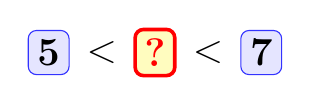
\begin{tikzpicture}[scale=0.75, baseline=(current bounding box.center)]
  \node[draw=blue!80, fill=blue!10, rounded corners=3pt, font=\Large\bfseries] at (-1.8,0) {5};
  \node[font=\Large\bfseries] at (-0.9,0) {$<$};
  \node[draw=red, fill=yellow!25, line width=1.3pt, rounded corners=3pt, font=\Large\bfseries, text=red] at (0,0) {?};
  \node[font=\Large\bfseries] at (0.9,0) {$<$};
  \node[draw=blue!80, fill=blue!10, rounded corners=3pt, font=\Large\bfseries] at (1.8,0) {7};
\end{tikzpicture}
\end{center}
\choice
{$5$}
{$7$}
{$8$}
{\True $6$}
\loigiai{
Số lớn hơn 5 và bé hơn 7 là số $6$ ($5 < 6 < 7$).\\
\textbf{Đáp án của câu hỏi là D}
}
\end{ex}

% --- CÂU 11 ---
\begin{ex} %[1D1V04]
Trong các số $5, 2, 4, 7$, số nào \textbf{bé hơn 3}?
\begin{center}
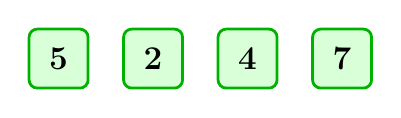
\begin{tikzpicture}[scale=0.75, baseline=(current bounding box.center)]
  \foreach \i/\num in {0/5, 1/2, 2/4, 3/7} {
    \draw[fill=green!15, draw=green!70!black, line width=1pt, rounded corners=3pt] (\i*1.6,-0.4) rectangle (\i*1.6+1.0,0.6);
    \node[font=\large\bfseries] at (\i*1.6+0.5, 0.1) {\num};
  }
\end{tikzpicture}
\end{center}
\choice
{$5$}
{\True $2$}
{$4$}
{$7$}
\loigiai{
Chỉ có số $2$ là bé hơn $3$ ($2 < 3$).\\
\textbf{Đáp án của câu hỏi là B}
}
\end{ex}

% --- CÂU 12 ---
\begin{ex} %[1D1C04]
Trong các số $0, 1, 2, 3, 4, 5$, có bao nhiêu số \textbf{bé hơn 4}?
\begin{center}
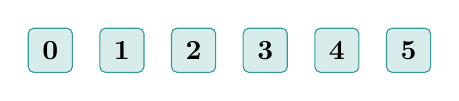
\begin{tikzpicture}[scale=0.7, baseline=(current bounding box.center)]
  \foreach \i in {0,1,2,3,4,5} {
    \draw[fill=teal!15, draw=teal!80, rounded corners=2pt] (\i*1.3,-0.3) rectangle (\i*1.3+0.8,0.5);
    \node[font=\bfseries] at (\i*1.3+0.4, 0.1) {\i};
  }
\end{tikzpicture}
\end{center}
\choice
{\True $4$ số}
{$3$ số}
{$5$ số}
{$6$ số}
\loigiai{
Các số bé hơn 4 là: $0, 1, 2, 3$ (gồm đúng $4$ số).\\
\textbf{Đáp án của câu hỏi là A}
}
\end{ex}

% =========================================================================
% PHẦN 2: TRẮC NGHIỆM ĐÚNG SAI (QUAN SÁT TRANH MINH HỌA)
% =========================================================================
\textbf{Phần 2. Trắc nghiệm đúng sai (Xét tính đúng/sai của các phép so sánh)}
\setcounterpageref{ex}{0}

% --- CÂU 13 ---
\begin{ex} %[1D1H04]
Xét tính đúng sai của các phép so sánh dưới đây:
\choiceTF
{\True $6 > 4$}
{\True $3 < 8$}
{$9 < 7$}
{\True $5 = 5$}
\loigiai{
\begin{itemize}
    \item $6 > 4$: \textbf{Đúng}.
    \item $3 < 8$: \textbf{Đúng}.
    \item $9 < 7$ là sai vì $9 > 7$: \textbf{Sai}.
    \item $5 = 5$: \textbf{Đúng}.
\end{itemize}
}
\end{ex}

% --- CÂU 14 ---
\begin{ex} %[1D1V04]
Cho nhóm các số: $2, 5, 8, 10$. Xét tính đúng sai của các câu sau:
\choiceTF
{\True Số lớn nhất trong nhóm là $10$.}
{\True Số bé nhất trong nhóm là $2$.}
{Số $5$ lớn hơn số $8$.}
{\True Số $8$ bé hơn số $10$.}
\loigiai{
\begin{itemize}
    \item Lớn nhất là $10$: \textbf{Đúng}.
    \item Bé nhất là $2$: \textbf{Đúng}.
    \item $5$ bé hơn $8$ (nói lớn hơn là sai): \textbf{Sai}.
    \item $8 < 10$: \textbf{Đúng}.
\end{itemize}
}
\end{ex}

% =========================================================================
% PHẦN 3: TRẢ LỜI NGẮN (ĐIỀN SỐ HOẶC DẤU THÍCH HỢP)
% =========================================================================
\textbf{Phần 3. Trả lời ngắn (Quan sát và điền đáp án thích hợp)}
\setcounterpageref{ex}{0}

% --- CÂU 15 ---
\begin{ex} %[1D1H04]
Điền dấu thích hợp ($>$, $<$, $=$) vào ô trống: $6 \dots 2$.
\shortans{>}
\loigiai{
\textbf{Đáp số:} $>$\\
Vì $6 > 2$.
}
\end{ex}

% --- CÂU 16 ---
\begin{ex} %[1D1H04]
Điền dấu thích hợp ($>$, $<$, $=$) vào ô trống: $7 \dots 10$.
\shortans{<}
\loigiai{
\textbf{Đáp số:} $<$\\
Vì $7 < 10$.
}
\end{ex}

% --- CÂU 17 ---
\begin{ex} %[1D1V04]
Tìm số thích hợp điền vào ô trống: $4 < \dots < 6$.
\shortans{5}
\loigiai{
\textbf{Đáp số:} $5$\\
Số ở giữa 4 và 6 là $5$.
}
\end{ex}

% --- CÂU 18 ---
\begin{ex} %[1D1V04]
Trong các số $8, 3, 9, 5$, số lớn nhất là số nào?
\shortans{9}
\loigiai{
\textbf{Đáp số:} $9$\\
Số lớn nhất là $9$.
}
\end{ex}

% --- CÂU 19 ---
\begin{ex} %[1D1V04]
Trong các số $6, 10, 4, 7$, số bé nhất là số nào?
\shortans{4}
\loigiai{
\textbf{Đáp số:} $4$\\
Số bé nhất là $4$.
}
\end{ex}

% --- CÂU 20 ---
\begin{ex} %[1D1C04]
Có bao nhiêu số lớn hơn $6$ và bé hơn $10$?
\shortans{3}
\loigiai{
\textbf{Đáp số:} $3$\\
Có 3 số là: $7, 8, 9$.
}
\end{ex}
